\documentclass[aspectratio=169]{beamer}
\usepackage[utf8]{inputenc}
\usepackage{graphicx}
\usepackage{listings}
\usepackage{xcolor}
\usepackage{tikz}
\usepackage{hyperref}

% Theme
\usetheme{Madrid}
\usecolortheme{default}

% Colors
\definecolor{reactblue}{RGB}{0,122,255}
\definecolor{codegreen}{RGB}{52,199,89}
\definecolor{codegray}{RGB}{102,102,102}
\definecolor{codepurple}{RGB}{175,0,219}
\definecolor{backcolour}{RGB}{245,245,245}

% Code style
\lstdefinestyle{mystyle}{
    backgroundcolor=\color{backcolour},
    commentstyle=\color{codegreen},
    keywordstyle=\color{reactblue},
    numberstyle=\tiny\color{codegray},
    stringstyle=\color{codepurple},
    basicstyle=\ttfamily\footnotesize,
    breakatwhitespace=false,
    breaklines=true,
    captionpos=b,
    keepspaces=true,
    numbers=left,
    numbersep=5pt,
    showspaces=false,
    showstringspaces=false,
    showtabs=false,
    tabsize=2
}
\lstset{style=mystyle}

% Title Page
\title{React Native}
\subtitle{End-to-End Mobile Development}
\author{Your Name}
\date{\today}
\institute{2-Hour Comprehensive Session}

\begin{document}

% ============================================
% TITLE SLIDE
% ============================================
\begin{frame}
\titlepage
\end{frame}

% ============================================
% TABLE OF CONTENTS
% ============================================
\begin{frame}{Agenda}
\tableofcontents
\end{frame}

% ============================================
% SECTION 1: INTRODUCTION
% ============================================
\section{Introduction to React Native}

\begin{frame}{What is React Native?}
\begin{columns}
\column{0.5\textwidth}
\textbf{Definition:}
\begin{itemize}
    \item Framework for building mobile apps
    \item Uses JavaScript and React
    \item Created by Facebook (Meta) in 2015
    \item Write once, run on iOS \& Android
    \item Real native apps, not hybrid
\end{itemize}

\column{0.5\textwidth}
\begin{center}
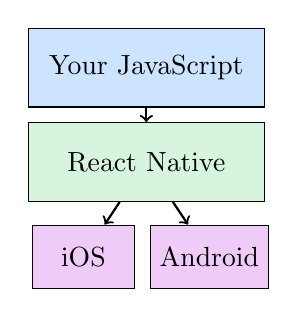
\begin{tikzpicture}[scale=0.8]
\node[draw, rectangle, fill=reactblue!20, minimum width=3cm, minimum height=1cm] (js) at (0,2) {Your JavaScript};
\node[draw, rectangle, fill=codegreen!20, minimum width=3cm, minimum height=1cm] (rn) at (0,0.5) {React Native};
\node[draw, rectangle, fill=codepurple!20, minimum width=1.3cm, minimum height=0.8cm] (ios) at (-1,-1) {iOS};
\node[draw, rectangle, fill=codepurple!20, minimum width=1.3cm, minimum height=0.8cm] (android) at (1,-1) {Android};
\draw[->, thick] (js) -- (rn);
\draw[->, thick] (rn) -- (ios);
\draw[->, thick] (rn) -- (android);
\end{tikzpicture}
\end{center}
\end{columns}

\vspace{0.5cm}
\textbf{Analogy:} React Native is a translator - you speak JavaScript, it speaks Swift/Kotlin to the phone
\end{frame}

\begin{frame}{How React Native Works}
\begin{center}
\textbf{The Bridge Architecture}
\end{center}

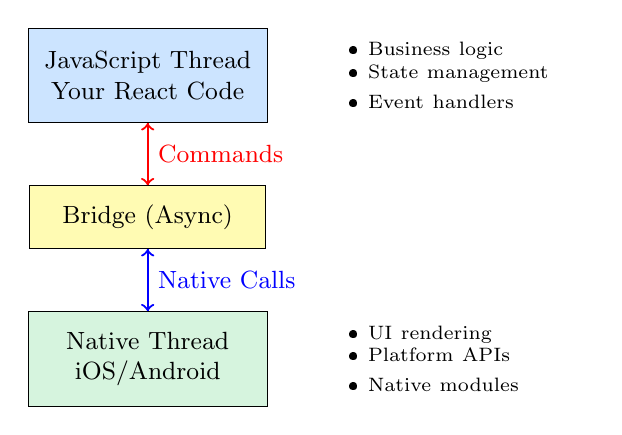
\begin{tikzpicture}[scale=0.9, every node/.style={font=\small}]
% JavaScript Thread
\node[draw, rectangle, fill=reactblue!20, minimum width=3cm, minimum height=1.2cm, text width=2.8cm, align=center] (js) at (0,4) {JavaScript Thread\\Your React Code};

% Bridge
\node[draw, rectangle, fill=yellow!30, minimum width=3cm, minimum height=0.8cm] (bridge) at (0,2) {Bridge (Async)};

% Native Thread
\node[draw, rectangle, fill=codegreen!20, minimum width=3cm, minimum height=1.2cm, text width=2.8cm, align=center] (native) at (0,0) {Native Thread\\iOS/Android};

\draw[->, thick, red] (js) -- (bridge) node[midway, right] {Commands};
\draw[->, thick, blue] (bridge) -- (native) node[midway, right] {Native Calls};
\draw[->, thick, blue] (native) -- (bridge);
\draw[->, thick, red] (bridge) -- (js);

% Side annotations
\node[text width=3cm, align=left] at (4.5,4) {\scriptsize • Business logic\\• State management\\• Event handlers};
\node[text width=3cm, align=left] at (4.5,0) {\scriptsize • UI rendering\\• Platform APIs\\• Native modules};
\end{tikzpicture}

\begin{block}{Key Concepts}
\begin{itemize}
    \item \textbf{Asynchronous:} Bridge is non-blocking
    \item \textbf{Batching:} Updates are batched for performance
    \item \textbf{Virtual DOM:} React calculates minimal changes
\end{itemize}
\end{block}
\end{frame}

\begin{frame}{How It Works - Step by Step}
\begin{enumerate}
    \item \textbf{You write JSX:}
    \begin{lstlisting}[language=JavaScript]
<View style={styles.container}>
  <Text>Hello!</Text>
</View>
    \end{lstlisting}

    \vspace{0.3cm}
    \item \textbf{React Native translates:}
    \begin{itemize}
        \item \texttt{<View>} → iOS: \texttt{UIView} / Android: \texttt{ViewGroup}
        \item \texttt{<Text>} → iOS: \texttt{UILabel} / Android: \texttt{TextView}
    \end{itemize}

    \vspace{0.3cm}
    \item \textbf{Bridge sends instructions} to native side

    \vspace{0.3cm}
    \item \textbf{Native code renders} actual components

    \vspace{0.3cm}
    \item \textbf{User interaction} → Event → Bridge → JavaScript → Update
\end{enumerate}
\end{frame}

\begin{frame}{The New Architecture (2024+)}
\begin{columns}
\column{0.5\textwidth}
\textbf{Old Architecture:}
\begin{itemize}
    \item Bridge (async, JSON)
    \item Performance overhead
    \item Serialization bottleneck
\end{itemize}

\column{0.5\textwidth}
\textbf{New Architecture:}
\begin{itemize}
    \item \textcolor{codegreen}{JSI} - JavaScript Interface
    \item \textcolor{codegreen}{Fabric} - New renderer
    \item \textcolor{codegreen}{TurboModules} - Lazy loading
    \item Direct C++ communication
\end{itemize}
\end{columns}

\vspace{0.5cm}
\begin{alertblock}{Impact}
Faster performance, synchronous rendering, better debugging
\end{alertblock}
\end{frame}

% ============================================
% SECTION 2: USE CASES
% ============================================
\section{What We Do With React Native}

\begin{frame}{Real-World Success Stories}
\begin{columns}
\column{0.5\textwidth}
\textbf{Apps Built with RN:}
\begin{itemize}
    \item 📱 Instagram (99\% shared code)
    \item 💬 Discord (60 FPS scrolling)
    \item 🛍️ Shopify (Complex features)
    \item 🍔 Uber Eats (Real-time tracking)
    \item 📘 Facebook (Where it started)
    \item 🎵 SoundCloud
\end{itemize}

\column{0.5\textwidth}
\textbf{When to Use RN:}
\begin{itemize}
    \item ✅ Cross-platform apps
    \item ✅ Rapid prototyping
    \item ✅ JavaScript team
    \item ✅ Frequent updates
    \item ✅ Budget/time constraints
\end{itemize}

\vspace{0.5cm}
\textbf{When NOT to use:}
\begin{itemize}
    \item ❌ Heavy 3D graphics/games
    \item ❌ Maximum performance critical
    \item ❌ Platform-specific features only
\end{itemize}
\end{columns}
\end{frame}

% ============================================
% SECTION 3: SETUP
% ============================================
\section{Development Setup}

\begin{frame}[fragile]{Prerequisites \& Installation}
\begin{columns}
\column{0.5\textwidth}
\textbf{Required Software:}
\begin{itemize}
    \item Node.js (v16+)
    \item npm/npx
    \item Code editor (VS Code)
    \item For iOS: Mac + Xcode
    \item For Android: Android Studio
\end{itemize}

\column{0.5\textwidth}
\textbf{Verify Installation:}
\begin{lstlisting}[language=bash]
node --version
npm --version
npx --version
\end{lstlisting}
\end{columns}

\vspace{0.5cm}
\textbf{Development Approaches:}
\begin{itemize}
    \item \textbf{Expo} (Recommended): Managed workflow, quick setup
    \item \textbf{React Native CLI}: Full control, more complex
\end{itemize}
\end{frame}

\begin{frame}[fragile]{npm vs npx}
\begin{columns}
\column{0.5\textwidth}
\textbf{npm (Package Manager):}
\begin{lstlisting}[language=bash]
# Install package
npm install package-name

# Install globally
npm install -g package-name

# Run script
npm run start
\end{lstlisting}

\column{0.5\textwidth}
\textbf{npx (Package Executor):}
\begin{lstlisting}[language=bash]
# Execute without installing
npx create-expo-app MyApp

# Always uses latest
npx react-native init App
\end{lstlisting}
\end{columns}

\vspace{0.5cm}
\begin{block}{Why npx?}
\begin{itemize}
    \item No global installation needed
    \item Always uses latest version
    \item Saves disk space
\end{itemize}
\end{block}
\end{frame}

% ============================================
% SECTION 4: CORE CONCEPTS
% ============================================
\section{Core Concepts}

\begin{frame}{Component Mapping: Web vs Native}
\begin{center}
\begin{tabular}{|l|l|}
\hline
\textbf{React (Web)} & \textbf{React Native} \\
\hline
\texttt{<div>} & \texttt{<View>} \\
\texttt{<span>}, \texttt{<p>} & \texttt{<Text>} \\
\texttt{<img>} & \texttt{<Image>} \\
\texttt{<input>} & \texttt{<TextInput>} \\
\texttt{<button>} & \texttt{<Button>} / \texttt{<TouchableOpacity>} \\
\texttt{<ul>}, \texttt{<li>} & \texttt{<FlatList>} \\
\texttt{<scroll>} & \texttt{<ScrollView>} \\
\hline
\end{tabular}
\end{center}

\vspace{0.5cm}
\begin{alertblock}{Key Difference}
No HTML in React Native! Everything is a React component.
\end{alertblock}
\end{frame}

\begin{frame}{React vs React Native}
\begin{center}
\begin{tabular}{|l|l|l|}
\hline
\textbf{Aspect} & \textbf{React (Web)} & \textbf{React Native} \\
\hline
Platform & Browsers & iOS \& Android \\
Elements & HTML tags & Native components \\
Styling & CSS files & StyleSheet objects \\
Layout & CSS Box Model & Flexbox (default) \\
Navigation & React Router & React Navigation \\
Bundler & Webpack/Vite & Metro \\
Runtime & Browser DOM & Native + JS threads \\
\hline
\end{tabular}
\end{center}

\vspace{0.5cm}
\textbf{Similarities:}
\begin{itemize}
    \item ✅ Same React principles (components, props, state, hooks)
    \item ✅ Same lifecycle methods
    \item ✅ JSX syntax
\end{itemize}
\end{frame}

\begin{frame}[fragile]{Styling in React Native}
\begin{columns}
\column{0.5\textwidth}
\textbf{No CSS Files!}
\begin{itemize}
    \item JavaScript objects
    \item StyleSheet.create()
    \item Flexbox by default
    \item No pixels (density-independent)
\end{itemize}

\column{0.5\textwidth}
\begin{lstlisting}[language=JavaScript]
const styles = StyleSheet.create({
  container: {
    flex: 1,
    backgroundColor: '#fff',
    alignItems: 'center',
    justifyContent: 'center',
  },
  title: {
    fontSize: 24,
    fontWeight: 'bold',
    color: '#333',
  },
});
\end{lstlisting}
\end{columns}

\vspace{0.5cm}
\begin{block}{Flexbox Properties}
\texttt{flexDirection}, \texttt{justifyContent}, \texttt{alignItems}, \texttt{flex}, \texttt{padding}, \texttt{margin}
\end{block}
\end{frame}

% ============================================
% SECTION 5: BUILDING THE APP
% ============================================
\section{Building Our Progressive App}

\begin{frame}{The Journey - One App, Four Versions}
\begin{center}
\begin{tikzpicture}[scale=0.85]
% Version 1
\node[draw, circle, fill=reactblue!30, minimum size=1.5cm] (v1) at (0,0) {V1};
\node[below=0.1cm of v1] {\small Basic App};

% Arrow
\draw[->, thick] (1,0) -- (2.5,0);

% Version 2
\node[draw, circle, fill=codegreen!30, minimum size=1.5cm] (v2) at (4,0) {V2};
\node[below=0.1cm of v2] {\small + Tabs};

% Arrow
\draw[->, thick] (5,0) -- (6.5,0);

% Version 3
\node[draw, circle, fill=yellow!50, minimum size=1.5cm] (v3) at (8,0) {V3};
\node[below=0.1cm of v3] {\small + Notifications};

% Arrow
\draw[->, thick] (9,0) -- (10.5,0);

% Version 4
\node[draw, circle, fill=codepurple!30, minimum size=1.5cm] (v4) at (12,0) {V4};
\node[below=0.1cm of v4] {\small + Props/Redux};
\end{tikzpicture}
\end{center}

\vspace{0.5cm}
\textbf{Learning Path:}
\begin{enumerate}
    \item Start simple → Build foundation
    \item Add navigation → Multiple screens
    \item Add complexity → Real features
    \item Add state management → Scale up
\end{enumerate}
\end{frame}

\begin{frame}[fragile]{VERSION 1: Basic App}
\textbf{What We'll Build:}
\begin{itemize}
    \item Welcome screen
    \item Counter with buttons
    \item Styling with StyleSheet
    \item State management with useState
\end{itemize}

\vspace{0.3cm}
\textbf{Concepts Covered:}
\begin{itemize}
    \item Components: View, Text, TouchableOpacity, Image
    \item State: useState hook
    \item Events: onPress handlers
    \item Styling: StyleSheet.create, Flexbox
\end{itemize}

\vspace{0.3cm}
\begin{lstlisting}[language=bash]
# Create the app
npx create-expo-app MyApp
cd MyApp
npx expo start --android
\end{lstlisting}
\end{frame}

\begin{frame}[fragile]{VERSION 1: Code Structure}
\begin{lstlisting}[language=JavaScript, basicstyle=\ttfamily\tiny]
import { useState } from 'react';
import { View, Text, TouchableOpacity, StyleSheet } from 'react-native';

export default function App() {
  const [count, setCount] = useState(0);

  return (
    <View style={styles.container}>
      <Text style={styles.title}>Welcome to React Native!</Text>

      <View style={styles.counterBox}>
        <Text style={styles.counterValue}>{count}</Text>

        <TouchableOpacity
          style={styles.button}
          onPress={() => setCount(count + 1)}>
          <Text style={styles.buttonText}>Increment</Text>
        </TouchableOpacity>

        <TouchableOpacity
          style={styles.button}
          onPress={() => setCount(0)}>
          <Text style={styles.buttonText}>Reset</Text>
        </TouchableOpacity>
      </View>
    </View>
  );
}
\end{lstlisting}
\end{frame}

\begin{frame}{VERSION 1: Key Learnings}
\begin{block}{Components}
\begin{itemize}
    \item \texttt{<View>} is like \texttt{<div>} - a container
    \item \texttt{<Text>} for all text (can't put text directly in View!)
    \item \texttt{<TouchableOpacity>} for touchable elements
\end{itemize}
\end{block}

\begin{block}{State}
\begin{itemize}
    \item \texttt{useState()} creates state variable
    \item State updates trigger re-render
    \item Always use setter function: \texttt{setCount(newValue)}
\end{itemize}
\end{block}

\begin{block}{Styling}
\begin{itemize}
    \item \texttt{StyleSheet.create()} for optimization
    \item Camel case: \texttt{backgroundColor}, \texttt{fontSize}
    \item No units: 20 not "20px"
\end{itemize}
\end{block}
\end{frame}

\begin{frame}[fragile]{VERSION 2: Adding Tab Navigation}
\textbf{Evolution:}
\begin{itemize}
    \item Keep counter from V1
    \item Add multiple screens (Home, Profile, Settings)
    \item Add bottom tab navigation
    \item Add icons for tabs
\end{itemize}

\vspace{0.3cm}
\textbf{New Dependencies:}
\begin{lstlisting}[language=bash, basicstyle=\ttfamily\scriptsize]
npm install @react-navigation/native @react-navigation/bottom-tabs
npx expo install react-native-screens react-native-safe-area-context
\end{lstlisting}

\vspace{0.3cm}
\textbf{Concepts Added:}
\begin{itemize}
    \item React Navigation setup
    \item NavigationContainer
    \item createBottomTabNavigator
    \item Tab icons with Ionicons
    \item Screen components
\end{itemize}
\end{frame}

\begin{frame}[fragile]{VERSION 2: Navigation Setup}
\begin{lstlisting}[language=JavaScript, basicstyle=\ttfamily\tiny]
import { NavigationContainer } from '@react-navigation/native';
import { createBottomTabNavigator } from '@react-navigation/bottom-tabs';
import { Ionicons } from '@expo/vector-icons';

const Tab = createBottomTabNavigator();

function HomeScreen() {
  // Counter code from V1
}

function ProfileScreen() {
  // New profile screen
}

export default function App() {
  return (
    <NavigationContainer>
      <Tab.Navigator screenOptions={({ route }) => ({
        tabBarIcon: ({ focused, color, size }) => {
          let iconName = route.name === 'Home'
            ? (focused ? 'home' : 'home-outline')
            : (focused ? 'person' : 'person-outline');
          return <Ionicons name={iconName} size={size} color={color} />;
        },
      })}>
        <Tab.Screen name="Home" component={HomeScreen} />
        <Tab.Screen name="Profile" component={ProfileScreen} />
      </Tab.Navigator>
    </NavigationContainer>
  );
}
\end{lstlisting}
\end{frame}

\begin{frame}{VERSION 2: Key Learnings}
\begin{block}{Navigation}
\begin{itemize}
    \item \texttt{NavigationContainer} wraps entire app
    \item Each screen is a separate component
    \item Tab navigator manages screen switching
    \item Icons change based on \texttt{focused} state
\end{itemize}
\end{block}

\begin{block}{Screen Organization}
\begin{itemize}
    \item Separate function for each screen
    \item Each screen has its own state
    \item Shared styles across screens
    \item Can navigate programmatically: \texttt{navigation.navigate('ScreenName')}
\end{itemize}
\end{block}

\begin{block}{Icons}
\begin{itemize}
    \item Expo includes Ionicons by default
    \item Search icons at: icons.expo.fyi
    \item Outline version for inactive, solid for active
\end{itemize}
\end{block}
\end{frame}

\begin{frame}[fragile]{VERSION 3: Adding Notifications}
\textbf{Evolution:}
\begin{itemize}
    \item Add Notifications tab
    \item List of notifications with FlatList
    \item Mark as read/unread
    \item Delete notifications
    \item Show unread count
\end{itemize}

\vspace{0.3cm}
\textbf{New Components:}
\begin{itemize}
    \item \texttt{<FlatList>} for efficient lists
    \item \texttt{Alert} API for confirmations
    \item More complex state (array of objects)
    \item Array methods: map, filter, find
\end{itemize}

\vspace{0.3cm}
\textbf{Concepts Added:}
\begin{itemize}
    \item Lists and keys
    \item Complex state management
    \item User interactions (tap, long press)
    \item Conditional rendering
    \item Immutable state updates
\end{itemize}
\end{frame}

\begin{frame}[fragile]{VERSION 3: FlatList Implementation}
\begin{lstlisting}[language=JavaScript, basicstyle=\ttfamily\tiny]
function NotificationsScreen() {
  const [notifications, setNotifications] = useState([
    { id: '1', title: 'Welcome!', message: 'Thanks for joining', read: false },
    { id: '2', title: 'New Update', message: 'Version 2.0', read: false },
  ]);

  const markAsRead = (id) => {
    setNotifications(
      notifications.map(notif =>
        notif.id === id ? { ...notif, read: true } : notif
      )
    );
  };

  const renderNotification = ({ item }) => (
    <TouchableOpacity
      style={[styles.card, item.read && styles.readCard]}
      onPress={() => markAsRead(item.id)}>
      <Text style={styles.title}>{item.title}</Text>
      <Text style={styles.message}>{item.message}</Text>
      {!item.read && <View style={styles.unreadDot} />}
    </TouchableOpacity>
  );

  return (
    <FlatList
      data={notifications}
      renderItem={renderNotification}
      keyExtractor={(item) => item.id}
    />
  );
}
\end{lstlisting}
\end{frame}

\begin{frame}{VERSION 3: Key Learnings}
\begin{block}{FlatList}
\begin{itemize}
    \item Use for long lists (not .map())
    \item \texttt{renderItem} function returns component
    \item \texttt{keyExtractor} for unique keys (required!)
    \item Virtualized - only renders visible items
    \item ListEmptyComponent for empty state
\end{itemize}
\end{block}

\begin{block}{Immutable State Updates}
\begin{itemize}
    \item ❌ Don't: \texttt{notifications.push(newItem)}
    \item ✅ Do: \texttt{setNotifications([...notifications, newItem])}
    \item Use spread operator \texttt{...} to create new array/object
    \item Array methods: \texttt{map()}, \texttt{filter()}
\end{itemize}
\end{block}

\begin{block}{User Interactions}
\begin{itemize}
    \item \texttt{onPress} for tap
    \item \texttt{onLongPress} for long press
    \item \texttt{Alert.alert()} for native dialogs
\end{itemize}
\end{block}
\end{frame}

\begin{frame}[fragile]{VERSION 4: Props \& Redux}
\textbf{Final Evolution:}
\begin{itemize}
    \item Extract components with props
    \item Share state with Redux
    \item Connect all screens to store
    \item Global notification count
\end{itemize}

\vspace{0.3cm}
\textbf{New Dependencies:}
\begin{lstlisting}[language=bash]
npm install @reduxjs/toolkit react-redux
\end{lstlisting}

\vspace{0.3cm}
\textbf{Concepts Added:}
\begin{itemize}
    \item Props: passing data to components
    \item Redux store: centralized state
    \item Slices: feature-based reducers
    \item useSelector: read from store
    \item useDispatch: send actions to store
\end{itemize}
\end{frame}

\begin{frame}[fragile]{VERSION 4: Props Example}
\begin{lstlisting}[language=JavaScript, basicstyle=\ttfamily\tiny]
// Child Component - receives props
function NotificationCard({ title, message, isRead, onPress }) {
  return (
    <TouchableOpacity
      style={[styles.card, isRead && styles.readCard]}
      onPress={onPress}>
      <Text style={styles.title}>{title}</Text>
      <Text style={styles.message}>{message}</Text>
      {!isRead && <View style={styles.unreadDot} />}
    </TouchableOpacity>
  );
}

// Parent Component - passes props
function NotificationList() {
  const [notifications, setNotifications] = useState([...]);

  return (
    <View>
      {notifications.map((notif) => (
        <NotificationCard
          key={notif.id}
          title={notif.title}
          message={notif.message}
          isRead={notif.read}
          onPress={() => markAsRead(notif.id)}
        />
      ))}
    </View>
  );
}
\end{lstlisting}
\end{frame}

\begin{frame}{Props: Data Flow}
\begin{center}
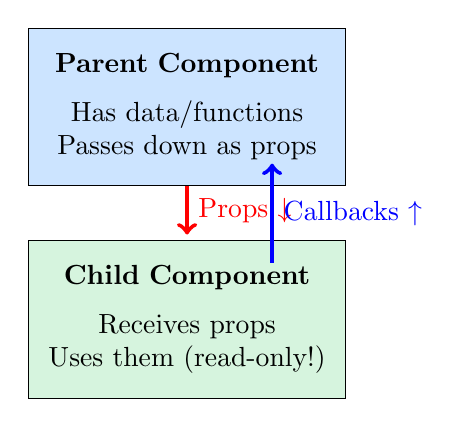
\begin{tikzpicture}[scale=0.9]
% Parent Component
\node[draw, rectangle, fill=reactblue!20, minimum width=4cm, minimum height=2cm, text width=3.8cm, align=center] (parent) at (0,3) {
    \textbf{Parent Component}\\
    \vspace{0.2cm}
    Has data/functions\\
    Passes down as props
};

% Arrow down
\draw[->, ultra thick, red] (parent) -- (0,1.2) node[midway, right] {Props $\downarrow$};

% Child Component
\node[draw, rectangle, fill=codegreen!20, minimum width=4cm, minimum height=2cm, text width=3.8cm, align=center] (child) at (0,0) {
    \textbf{Child Component}\\
    \vspace{0.2cm}
    Receives props\\
    Uses them (read-only!)
};

% Arrow up (callbacks)
\draw[->, ultra thick, blue] (1.2,0.8) -- (1.2,2.2) node[midway, right] {Callbacks $\uparrow$};
\end{tikzpicture}
\end{center}

\begin{alertblock}{Remember}
\begin{itemize}
    \item Props flow DOWN (parent → child)
    \item Events/Callbacks flow UP (child → parent)
    \item Props are READ-ONLY in child
\end{itemize}
\end{alertblock}
\end{frame}

\begin{frame}[fragile]{VERSION 4: Redux Setup}
\begin{lstlisting}[language=JavaScript, basicstyle=\ttfamily\tiny]
// store/notificationSlice.js
import { createSlice } from '@reduxjs/toolkit';

const notificationSlice = createSlice({
  name: 'notifications',
  initialState: {
    items: [],
    unreadCount: 0,
  },
  reducers: {
    addNotification: (state, action) => {
      state.items.push(action.payload);
      state.unreadCount += 1;
    },
    markAsRead: (state, action) => {
      const notif = state.items.find(item => item.id === action.payload);
      if (notif && !notif.read) {
        notif.read = true;
        state.unreadCount -= 1;
      }
    },
  },
});

export const { addNotification, markAsRead } = notificationSlice.actions;
export default notificationSlice.reducer;
\end{lstlisting}
\end{frame}

\begin{frame}[fragile]{VERSION 4: Using Redux}
\begin{lstlisting}[language=JavaScript, basicstyle=\ttfamily\tiny]
// In component
import { useSelector, useDispatch } from 'react-redux';
import { markAsRead } from './store/notificationSlice';

function NotificationsScreen() {
  // Read from store
  const notifications = useSelector(state => state.notifications.items);
  const unreadCount = useSelector(state => state.notifications.unreadCount);

  // Get dispatch function
  const dispatch = useDispatch();

  // Dispatch action
  const handleMarkAsRead = (id) => {
    dispatch(markAsRead(id));
  };

  return (
    <View>
      <Text>Unread: {unreadCount}</Text>
      <FlatList
        data={notifications}
        renderItem={({ item }) => (
          <NotificationCard
            {...item}
            onPress={() => handleMarkAsRead(item.id)}
          />
        )}
      />
    </View>
  );
}
\end{lstlisting}
\end{frame}

\begin{frame}{Redux: When to Use}
\begin{columns}
\column{0.5\textwidth}
\textbf{Use Redux when:}
\begin{itemize}
    \item State shared across many components
    \item Complex state logic
    \item Need predictable state updates
    \item Time-travel debugging
    \item Large applications
\end{itemize}

\column{0.5\textwidth}
\textbf{Don't use Redux if:}
\begin{itemize}
    \item Simple apps
    \item State only in 1-2 components
    \item Can use Context API
    \item Learning curve too steep
\end{itemize}
\end{columns}

\vspace{0.5cm}
\begin{center}
\textbf{Redux Flow}
\end{center}

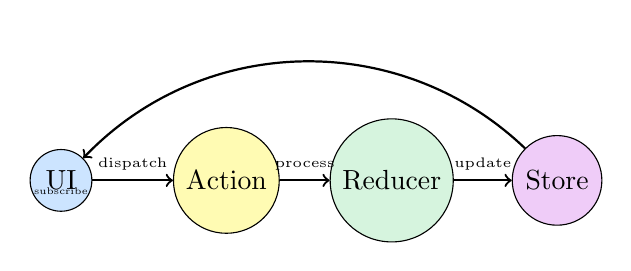
\begin{tikzpicture}[scale=0.7]
\node[draw, circle, fill=reactblue!20] (ui) at (0,0) {UI};
\node[draw, circle, fill=yellow!30] (action) at (3,0) {Action};
\node[draw, circle, fill=codegreen!20] (reducer) at (6,0) {Reducer};
\node[draw, circle, fill=codepurple!20] (store) at (9,0) {Store};

\draw[->, thick] (ui) -- (action) node[midway, above] {\tiny dispatch};
\draw[->, thick] (action) -- (reducer) node[midway, above] {\tiny process};
\draw[->, thick] (reducer) -- (store) node[midway, above] {\tiny update};
\draw[->, thick] (store) to[bend right=45] (ui) node[midway, below] {\tiny subscribe};
\end{tikzpicture}
\end{frame}

\begin{frame}{Call by Value vs Call by Reference}
\begin{columns}
\column{0.5\textwidth}
\textbf{Primitives (Value):}
\begin{itemize}
    \item Numbers, Strings, Booleans
    \item Copy is created
    \item Changing copy doesn't affect original
\end{itemize}

\begin{lstlisting}[language=JavaScript, basicstyle=\ttfamily\scriptsize]
let a = 5;
let b = a;  // b gets COPY
b = 10;     // a is still 5
\end{lstlisting}

\column{0.5\textwidth}
\textbf{Objects/Arrays (Reference):}
\begin{itemize}
    \item Objects, Arrays
    \item Reference is copied
    \item Changing reference affects original
\end{itemize}

\begin{lstlisting}[language=JavaScript, basicstyle=\ttfamily\scriptsize]
let obj1 = { name: 'John' };
let obj2 = obj1;  // REFERENCE
obj2.name = 'Jane';
// obj1.name is now 'Jane'!
\end{lstlisting}
\end{columns}

\vspace{0.5cm}
\begin{alertblock}{React Best Practice}
Always create new objects/arrays when updating state:
\begin{lstlisting}[language=JavaScript, basicstyle=\ttfamily\scriptsize]
// Correct
setUser({ ...user, name: 'New Name' });
setItems([...items, newItem]);
\end{lstlisting}
\end{alertblock}
\end{frame}

% ============================================
% SECTION 6: BEST PRACTICES
% ============================================
\section{Best Practices \& Common Mistakes}

\begin{frame}{Common Mistakes to Avoid}
\begin{block}{1. Mutating State Directly}
\textbf{❌ Wrong:}
\begin{lstlisting}[language=JavaScript, basicstyle=\ttfamily\scriptsize]
items.push(newItem);
setItems(items);  // Won't trigger re-render!
\end{lstlisting}

\textbf{✅ Correct:}
\begin{lstlisting}[language=JavaScript, basicstyle=\ttfamily\scriptsize]
setItems([...items, newItem]);  // New array
\end{lstlisting}
\end{block}

\begin{block}{2. Missing Keys in Lists}
\textbf{❌ Wrong:}
\begin{lstlisting}[language=JavaScript, basicstyle=\ttfamily\scriptsize]
{items.map(item => <Item item={item} />)}
\end{lstlisting}

\textbf{✅ Correct:}
\begin{lstlisting}[language=JavaScript, basicstyle=\ttfamily\scriptsize]
{items.map(item => <Item key={item.id} item={item} />)}
\end{lstlisting}
\end{block}
\end{frame}

\begin{frame}{Performance Tips}
\begin{enumerate}
    \item \textbf{Use FlatList} for long lists
    \begin{itemize}
        \item Virtualizes items
        \item Only renders visible items
        \item Much better than .map()
    \end{itemize}

    \vspace{0.3cm}
    \item \textbf{Memoize expensive components}
    \begin{itemize}
        \item Use React.memo() for components
        \item Use useCallback for functions
        \item Use useMemo for expensive calculations
    \end{itemize}

    \vspace{0.3cm}
    \item \textbf{Optimize images}
    \begin{itemize}
        \item Resize before loading
        \item Use appropriate formats
        \item Cache with FastImage library
    \end{itemize}

    \vspace{0.3cm}
    \item \textbf{Use StyleSheet.create()}
    \begin{itemize}
        \item Not inline styles
        \item Created once, reused
    \end{itemize}
\end{enumerate}
\end{frame}

% ============================================
% SECTION 7: SWIFT VS JAVASCRIPT
% ============================================
\section{Swift Fundamentals \& Comparison}

\begin{frame}{Why Learn Swift?}
\begin{columns}
\column{0.5\textwidth}
\textbf{Swift for iOS:}
\begin{itemize}
    \item Native iOS development
    \item Maximum performance
    \item Full platform access
    \item Official Apple language
    \item Growing ecosystem
\end{itemize}

\column{0.5\textwidth}
\textbf{When You Need Swift:}
\begin{itemize}
    \item iOS-specific features
    \item Deep system integration
    \item Native modules for RN
    \item Performance-critical code
    \item Apple Watch, CarPlay
\end{itemize}
\end{columns}

\vspace{0.5cm}
\begin{alertblock}{Good News}
If you know JavaScript, learning Swift is easier! Many similar concepts.
\end{alertblock}
\end{frame}

\begin{frame}{Swift vs JavaScript: Overview}
\begin{center}
\begin{tabular}{|l|l|l|}
\hline
\textbf{Feature} & \textbf{JavaScript} & \textbf{Swift} \\
\hline
Type System & Dynamic, loosely typed & Static, strongly typed \\
Compilation & Interpreted (JIT) & Compiled (AOT) \\
Platform & Cross-platform & Apple only \\
Performance & Good & Excellent \\
Learning Curve & Easier & Steeper \\
Syntax & C-style & Modern, clean \\
Memory & Garbage collected & ARC \\
\hline
\end{tabular}
\end{center}

\vspace{0.5cm}
\textbf{Key Difference:}
\begin{itemize}
    \item JavaScript: Flexible, dynamic, forgiving
    \item Swift: Strict, safe, explicit
\end{itemize}
\end{frame}

\begin{frame}[fragile]{Variables \& Constants}
\begin{columns}
\column{0.5\textwidth}
\textbf{JavaScript:}
\begin{lstlisting}[language=JavaScript, basicstyle=\ttfamily\scriptsize]
// Variable (can change)
let name = "John";
name = "Jane";  // OK

// Constant (can't change)
const age = 25;
age = 26;  // Error

// Type is inferred
let count = 5;  // number
\end{lstlisting}

\column{0.5\textwidth}
\textbf{Swift:}
\begin{lstlisting}[language=Swift, basicstyle=\ttfamily\scriptsize]
// Variable (can change)
var name = "John"
name = "Jane"  // OK

// Constant (can't change)
let age = 25
age = 26  // Error

// Type is inferred
let count = 5  // Int
// Or explicit type
let age: Int = 25
\end{lstlisting}
\end{columns}

\vspace{0.5cm}
\begin{block}{Similarity}
Both use \texttt{let} for constants! Swift uses \texttt{var}, JS uses \texttt{let} for variables.
\end{block}
\end{frame}

\begin{frame}[fragile]{Functions}
\begin{columns}
\column{0.5\textwidth}
\textbf{JavaScript:}
\begin{lstlisting}[language=JavaScript, basicstyle=\ttfamily\scriptsize]
// Function declaration
function greet(name) {
  return `Hello, ${name}!`;
}

// Arrow function
const greet = (name) => {
  return `Hello, ${name}!`;
};

// Short arrow
const greet = name =>
  `Hello, ${name}!`;

// Call
greet("John");  // "Hello, John!"
\end{lstlisting}

\column{0.5\textwidth}
\textbf{Swift:}
\begin{lstlisting}[language=Swift, basicstyle=\ttfamily\scriptsize]
// Function declaration
func greet(name: String) -> String {
  return "Hello, \(name)!"
}

// With parameter label
func greet(person name: String) -> String {
  return "Hello, \(name)!"
}

// Call
greet(name: "John")  // "Hello, John!"
greet(person: "John") // Same
\end{lstlisting}
\end{columns}

\vspace{0.5cm}
\textbf{Key Differences:}
\begin{itemize}
    \item Swift requires type annotations: \texttt{String}, \texttt{Int}, etc.
    \item Swift uses \texttt{->} for return type
    \item Swift has parameter labels
\end{itemize}
\end{frame}

\begin{frame}[fragile]{Arrays \& Dictionaries}
\begin{columns}
\column{0.5\textwidth}
\textbf{JavaScript:}
\begin{lstlisting}[language=JavaScript, basicstyle=\ttfamily\scriptsize]
// Array
let numbers = [1, 2, 3, 4, 5];
numbers.push(6);
numbers[0];  // 1

// Object (Dictionary)
let person = {
  name: "John",
  age: 25
};
person.name;  // "John"
person["age"];  // 25

// Methods
numbers.map(n => n * 2);
numbers.filter(n => n > 3);
\end{lstlisting}

\column{0.5\textwidth}
\textbf{Swift:}
\begin{lstlisting}[language=Swift, basicstyle=\ttfamily\scriptsize]
// Array
var numbers = [1, 2, 3, 4, 5]
numbers.append(6)
numbers[0]  // 1

// Dictionary
var person = [
  "name": "John",
  "age": 25
]
person["name"]  // Optional("John")

// Methods
numbers.map { $0 * 2 }
numbers.filter { $0 > 3 }
\end{lstlisting}
\end{columns}

\vspace{0.5cm}
\textbf{Swift Difference:} Dictionary values are Optionals (might be nil)
\end{frame}

\begin{frame}[fragile]{Optionals (Swift Unique Feature)}
\textbf{What are Optionals?}
\begin{itemize}
    \item A value that might be \texttt{nil} (nothing)
    \item Like JavaScript's \texttt{null} or \texttt{undefined}
    \item But explicit in the type system
\end{itemize}

\vspace{0.3cm}
\begin{columns}
\column{0.5\textwidth}
\textbf{JavaScript:}
\begin{lstlisting}[language=JavaScript, basicstyle=\ttfamily\scriptsize]
let name = null;
if (name) {
  console.log(name);
}

// Optional chaining
user?.profile?.name;
\end{lstlisting}

\column{0.5\textwidth}
\textbf{Swift:}
\begin{lstlisting}[language=Swift, basicstyle=\ttfamily\scriptsize]
var name: String? = nil

// Unwrap with if-let
if let name = name {
  print(name)
}

// Optional chaining
user?.profile?.name
\end{lstlisting}
\end{columns}

\vspace{0.5cm}
\begin{alertblock}{Safety}
Swift forces you to handle nil cases explicitly. Prevents crashes!
\end{alertblock}
\end{frame}

\begin{frame}[fragile]{Classes \& Structs}
\begin{columns}
\column{0.5\textwidth}
\textbf{JavaScript:}
\begin{lstlisting}[language=JavaScript, basicstyle=\ttfamily\tiny]
class Person {
  constructor(name, age) {
    this.name = name;
    this.age = age;
  }

  greet() {
    return `Hi, I'm ${this.name}`;
  }
}

const john = new Person("John", 25);
john.greet();  // "Hi, I'm John"
\end{lstlisting}

\column{0.5\textwidth}
\textbf{Swift:}
\begin{lstlisting}[language=Swift, basicstyle=\ttfamily\tiny]
struct Person {  // or class
  var name: String
  var age: Int

  func greet() -> String {
    return "Hi, I'm \(name)"
  }
}

let john = Person(name: "John", age: 25)
john.greet()  // "Hi, I'm John"
\end{lstlisting}
\end{columns}

\vspace{0.5cm}
\textbf{Swift has both:}
\begin{itemize}
    \item \textbf{struct}: Value type (copy), for data
    \item \textbf{class}: Reference type (pointer), for objects
\end{itemize}
\end{frame}

\begin{frame}[fragile]{Control Flow}
\begin{columns}
\column{0.5\textwidth}
\textbf{JavaScript:}
\begin{lstlisting}[language=JavaScript, basicstyle=\ttfamily\tiny]
// If-else
if (age >= 18) {
  console.log("Adult");
} else {
  console.log("Minor");
}

// Switch
switch (day) {
  case "Mon":
    console.log("Monday");
    break;
  default:
    console.log("Other");
}

// For loop
for (let i = 0; i < 5; i++) {
  console.log(i);
}

// For-of
for (let item of items) {
  console.log(item);
}
\end{lstlisting}

\column{0.5\textwidth}
\textbf{Swift:}
\begin{lstlisting}[language=Swift, basicstyle=\ttfamily\tiny]
// If-else
if age >= 18 {
  print("Adult")
} else {
  print("Minor")
}

// Switch (no break needed!)
switch day {
case "Mon":
  print("Monday")
default:
  print("Other")
}

// For loop
for i in 0..<5 {
  print(i)
}

// For-in
for item in items {
  print(item)
}
\end{lstlisting}
\end{columns}

\vspace{0.3cm}
\textbf{Swift Advantage:} No parentheses required, no break in switch!
\end{frame}

\begin{frame}{Swift vs JavaScript: Summary}
\begin{center}
\begin{tabular}{|p{3cm}|p{3.5cm}|p{3.5cm}|}
\hline
\textbf{Concept} & \textbf{JavaScript} & \textbf{Swift} \\
\hline
Variables & \texttt{let}, \texttt{const} & \texttt{var}, \texttt{let} \\
\hline
Types & Dynamic & Static, strong \\
\hline
Null values & \texttt{null}, \texttt{undefined} & \texttt{nil} with Optionals \\
\hline
Functions & Flexible syntax & Type-annotated \\
\hline
Arrays & \texttt{[1, 2, 3]} & \texttt{[1, 2, 3]} similar! \\
\hline
Objects & \texttt{\{key: value\}} & Dictionary or Struct \\
\hline
Classes & \texttt{class} keyword & \texttt{class} and \texttt{struct} \\
\hline
String interpolation & \texttt{\$\{value\}} & \texttt{\\(value)} \\
\hline
\end{tabular}
\end{center}

\vspace{0.5cm}
\textbf{Recommendation:}
\begin{itemize}
    \item Learn React Native first
    \item Build apps and get comfortable
    \item Then learn Swift for native modules or iOS-specific features
\end{itemize}
\end{frame}

\begin{frame}{Swift Resources}
\begin{block}{Official Resources}
\begin{itemize}
    \item Swift.org - Official documentation
    \item Swift Playgrounds - Interactive learning
    \item Apple Developer Documentation
    \item WWDC Videos
\end{itemize}
\end{block}

\begin{block}{Learning Paths}
\begin{itemize}
    \item Hacking with Swift (hackingwithswift.com)
    \item Stanford CS193p (SwiftUI course)
    \item Ray Wenderlich tutorials
    \item 100 Days of Swift
\end{itemize}
\end{block}

\begin{block}{Practice}
\begin{itemize}
    \item Swift Playgrounds app (iPad/Mac)
    \item LeetCode in Swift
    \item Build small iOS apps
\end{itemize}
\end{block}
\end{frame}

% ============================================
% SECTION 8: CONCLUSION
% ============================================
\section{Conclusion \& Next Steps}

\begin{frame}{What We Covered Today}
\begin{enumerate}
    \item ✅ \textbf{Introduction}
    \begin{itemize}
        \item What is React Native
        \item How it works (Bridge architecture)
        \item When to use it
    \end{itemize}

    \item ✅ \textbf{Core Concepts}
    \begin{itemize}
        \item Components, Props, State
        \item Styling with StyleSheet
        \item React vs React Native
    \end{itemize}

    \item ✅ \textbf{Building Progressive App}
    \begin{itemize}
        \item V1: Basic app with counter
        \item V2: Tab navigation
        \item V3: Notifications with FlatList
        \item V4: Props \& Redux
    \end{itemize}

    \item ✅ \textbf{Best Practices}
    \begin{itemize}
        \item Common mistakes
        \item Performance tips
    \end{itemize}

    \item ✅ \textbf{Swift Basics}
    \begin{itemize}
        \item Swift vs JavaScript
        \item When to learn Swift
    \end{itemize}
\end{enumerate}
\end{frame}

\begin{frame}{Your Learning Journey}
\begin{center}
\begin{tikzpicture}[scale=0.8]
% Today
\node[draw, rectangle, fill=codegreen!30, minimum width=2.5cm, minimum height=1.2cm] (today) at (0,3) {\textbf{TODAY}};
\node[below=0.1cm of today, text width=2.3cm, align=center] {\tiny Built 4 versions\\Learned concepts};

\draw[->, thick] (today) -- (0,1.5);

% This Week
\node[draw, rectangle, fill=yellow!30, minimum width=2.5cm, minimum height=1.2cm] (week) at (0,1) {\textbf{THIS WEEK}};
\node[below=0.1cm of week, text width=2.3cm, align=center] {\tiny Build own project\\Practice daily};

\draw[->, thick] (week) -- (3,1);

% This Month
\node[draw, rectangle, fill=reactblue!30, minimum width=2.5cm, minimum height=1.2cm] (month) at (5.5,1) {\textbf{THIS MONTH}};
\node[below=0.1cm of month, text width=2.3cm, align=center] {\tiny Complex apps\\Deploy to stores};

\draw[->, thick] (month) -- (5.5,-0.5);

% Future
\node[draw, rectangle, fill=codepurple!30, minimum width=2.5cm, minimum height=1.2cm] (future) at (5.5,-1.5) {\textbf{FUTURE}};
\node[below=0.1cm of future, text width=2.3cm, align=center] {\tiny Professional dev\\Contribute OSS};
\end{tikzpicture}
\end{center}
\end{frame}

\begin{frame}{Next Steps}
\begin{block}{Continue Learning}
\begin{itemize}
    \item Build a todo app from scratch
    \item Add features to our progressive app
    \item Explore React Navigation (Stack, Drawer)
    \item Learn TypeScript with React Native
\end{itemize}
\end{block}

\begin{block}{Resources}
\begin{itemize}
    \item Official Docs: reactnative.dev
    \item Expo Docs: docs.expo.dev
    \item React Navigation: reactnavigation.org
    \item Redux Toolkit: redux-toolkit.js.org
\end{itemize}
\end{block}

\begin{block}{Join Community}
\begin{itemize}
    \item React Native Discord
    \item Stack Overflow
    \item GitHub projects
    \item Reddit r/reactnative
\end{itemize}
\end{block}
\end{frame}

\begin{frame}{Project Ideas}
\textbf{Beginner:}
\begin{itemize}
    \item Todo List app
    \item Calculator
    \item Weather app (API integration)
    \item Notes app with AsyncStorage
\end{itemize}

\vspace{0.5cm}
\textbf{Intermediate:}
\begin{itemize}
    \item Chat app with Firebase
    \item E-commerce app
    \item Social media feed
    \item Recipe app with search
\end{itemize}

\vspace{0.5cm}
\textbf{Advanced:}
\begin{itemize}
    \item Real-time collaboration app
    \item Fitness tracker with animations
    \item Music player
    \item Navigation app with maps
\end{itemize}
\end{frame}

\begin{frame}{Thank You!}
\begin{center}
{\Huge Questions?}

\vspace{1cm}

\textbf{Contact Information:}\\
\vspace{0.3cm}
Email: your.email@example.com\\
GitHub: github.com/yourusername\\
LinkedIn: linkedin.com/in/yourprofile

\vspace{1cm}

\textbf{All code examples and guides available at:}\\
GitHub Repository Link

\vspace{1cm}

{\Large Keep Building! 🚀}
\end{center}
\end{frame}

\end{document}
